In this section, we empirically demonstrate the advantages of our proposed PIDformer approach across multiple tasks, including ImageNet classification~\cite{deng2009imagenet}, ADE20K image segmentation~\cite{zhou2018semantic}, and language modeling on WikiText-103~\cite{DBLP:conf/iclr/MerityX0S17}. Our objectives are to: (i) illustrate that PIDformer significantly outperforms the transformer baseline with softmax-attention across diverse tasks, (ii) highlight that the PID DeiT model exhibits significantly higher robustness than softmax attention under various adversarial attacks, and for out-of-distribution generalization, (iii) demonstrate that PID DeiT does not suffer from rank collapse in output representation.
Throughout our experiments, we compare the performance of our proposed models with baselines of the same configuration. For additional details regarding datasets, models, and training procedures, please refer to Appendix~\ref{secapp:experiments}.

\textbf{Object Classification on ImageNet.}
To demonstrate the advantage of our PIDformer, we compare it with the DeiT baseline~\cite{touvron2020deit} on the ImageNet image classification task. Our PID DeiT surpasses the DeiT baseline, as shown in Table~\ref{tab:attacks}. Notably, our model performs significantly better than the baseline under white-box attacks, including fast gradient sign method (FGSM)~\cite{dong2020benchmarking}, projected gradient descent method (PGD)~\cite{tramer2019adversarial}; score-based black-box attack method SPSA~\cite{pmlr-v80-uesato18a}; and sparse $L_1$ descent (SLD)~\cite{NEURIPS2019_5d4ae76f} method as well as noise-adding attack. Moreover, the last four rows of Table~\ref{tab:attacks} demonstrate that PID DeiT is consistently more robust than the DeiT baseline under other adversarial examples and out-of-distribution dataset, including the Imagenet-C (common data corruption and perturbations, such as adding noise and blurring the images)~\cite{hendrycks2019benchmarking}, Imagenet-A (adversarial examples)~\cite{hendrycks2021natural}, Imagenet-R (out of distribution generalization)~\cite{hendrycks2021many}, and Imagenet-O(out-of-distribution detection)~\cite{hendrycks2021natural} datasets. Furthermore, in Appendix~\ref{secapp:moreattacks}, we visualize the performance gap between PID DeiT and the baseline DeiT model under attacks with escalating perturbation levels. This result demonstrates the significant advantages PIDformer has over the baseline model in terms of robustness, further confirming the benefits of our model.
\begin{table}[t!]
\vspace{-2mm}
\centering
% \small
\caption{\small 
Evaluation of PID DeiT versus Softmax DeiT on the clean ImageNet validation set, as well as under various adversarial attacks and out-of-distribution datasets.
}
    \vspace{-1em}
    \color{black}
    \begin{center}
    \scalebox{0.9}{
    \begin{tabular}{ll|cc}
    \toprule
         Attack& Metric/Model & \it Softmax DeiT  & PID DeiT (\%)  \\
        \midrule
        Clean& Top-1 Acc (\%)  &  72.17 & \bf 73.13 \\
        & Top-5 Acc (\%)  &  91.02 & \bf 91.76 \\
         \hline\midrule
        FGSM& Top-1 Acc (\%)  & 33.64  & \bf 38.52 \\
        & Top-5 Acc (\%)  & 68.18  & \bf 72.53 \\
         \hline%\midrule
        PGD& Top-1 Acc (\%)  & 12.02  & \bf 15.08 \\
        & Top-5 Acc (\%)  & 34.99  & \bf 39.69 \\
         \hline%\midrule
        SPSA& Top-1 Acc (\%)  & 65.75  & \bf67.98\bf  \\
        & Top-5 Acc (\%)  & 90.07  & \bf 90.58 \\
         \hline%\midrule
        SLD& Top-1 Acc (\%)  & 69.32  & \bf 70.84 \\
        & Top-5 Acc (\%)  & 90.8  & \bf 91.43 \\
         \hline%\midrule
        Noise & Top-1 Acc (\%)  & 69.2  & \bf 70.87 \\
        & Top-5 Acc (\%)  & 89.67  &\bf 90.77 \\
         \hline\midrule
         Imagenet-A & Top-1 Acc (\%)  & 6.90  & \bf 8.82 \\
         Imagenet-R & Top-1 Acc (\%)  & 32.83  & \bf 34.89 \\
         Imagenet-C & mCE ($\downarrow$)  & 71.20  & \bf 68.41 \\
         Imagenet-O & AUPR   & 17.47  & \bf 19.22 \\
        \bottomrule
    \end{tabular}}
    \end{center}
\vspace{-2mm}
\label{tab:attacks}
\end{table}

\textbf{Image Segmentation on ADE20K dataset.}
We evaluate the performance of Segmenter models \cite{strudel2021segmenter} using both PID DeiT and DeiT backbones on the ADE20K image segmentation task \cite{zhou2017scene}, as outlined in Table \ref{tab:segment}. The outcomes illustrate significant performance enhancements obtained by employing the PID DeiT backbone instead of the DeiT backbone across both single-scale (SS) and multi-scale (MS) Mean Intersection over Union (MIoU) metrics. 
\begin{table}[t!]
\vspace{-5mm}
\centering
% \small
\caption{\small 
\small 
Single-scale (SS) MIoU and multi-scale MIoU (MS) of the PID DeiT vs. the DeiT on the ADE20K image segmentation. 
}
    % \vspace{-0.5em}
    \color{black}
    \begin{center}
    \scalebox{0.9}{
    \begin{tabular}{l|cc}
    \toprule
         Model/Metric & SS MIoU  & MS MIoU (\%)  \\
        \midrule
        \it Softmax DeiT  &  35.72 & 36.68 \\
         % \hline  
        PID DeiT & \bf 37.42 & \bf 38.28 \\
        \bottomrule
    \end{tabular}}
    \end{center}
\label{tab:segment}
\end{table}

\textbf{Language Model on WikiText-103.}
In addition to computer vision tasks, we evaluate our model's performance in the language modeling task on the WikiText-103 dataset (Table~\ref{tab:lm}). Our PIDformer language model surpasses the softmax transformer model \cite{xiong2021nystromformer} in test and valid perplexity. These results, combined with findings across various tasks, empirically demonstrate the significant advantages of PIDformer models.
% Besides computer vision tasks, we also assess the performance of our model in a large-scale natural language processing application, particularly language modeling on the WikiText-103 dataset (see Table~\ref{tab:lm}). Our PIDformer language model outperforms the softmax transformer language model \cite{xiong2021nystromformer} in terms of both test perplexity and valid perplexity. These results, along with the outcomes observed across different tasks, provide empirical evidence of the considerable advantages offered by our PIDformer models.
\begin{table}[t!]
\vspace{-4mm}
\footnotesize
    \caption{\small Test and valid perplexity (Test PPL and Valid PPL) on WikiText-103 of PIDformer compared to the softmax transformer.% Our proposed method achieves a  significantly better performance PPL than the baseline.
    }
    % \vspace{-1em}
    \begin{center}
    \scalebox{1.}{
    \begin{tabular}{l|cc}
    \toprule
        Method/Metric & Valid PPL & Test PPL \\
        \midrule
        {\it Softmax Transformer} & 33.15  & 34.29 \\
         % \hline \hline 
        PIDformer & \bf 32.44  & \bf 33.45  \\
        \bottomrule
    \end{tabular}}
    \end{center}
% \vspace{-0.1in}
\label{tab:lm}
\end{table}

\textbf{Representation Collapse Analysis.}
We empirically show PIDformer's effectiveness in addressing rank collapse in transformers. In Fig.~\ref{fig:pid-cossim}, we compare token representation cosine similarity across layers in PID DeiT and softmax baseline models pretrained on Imagenet. PID DeiT exhibits significantly lower similarity, especially in later layers, alleviating rank collapse and enhancing token embedding diversity. Further details are in Appendix~\ref{secapp:cossim}.
% We provide empirical evidence demonstrating the efficacy of PIDformer in addressing the rank-collapse issue observed in transformers. In Fig.~\ref{fig:pid-cossim}, we compare the cosine similarity between token representations across layers for PID DeiT and softmax baseline models, which were pre-trained on the Imagenet classification task. Our results show that token features extracted by PID DeiT exhibit notably lower similarity, particularly in the final layers. This observation underscores the capability of PIDformer to alleviate the rank collapse problem in output representation and enhance the diversity of token embeddings. Additional details of this analysis are available in Appendix~\ref{secapp:cossim}.
\begin{figure}[!t]
\vspace{-5mm}
\centering
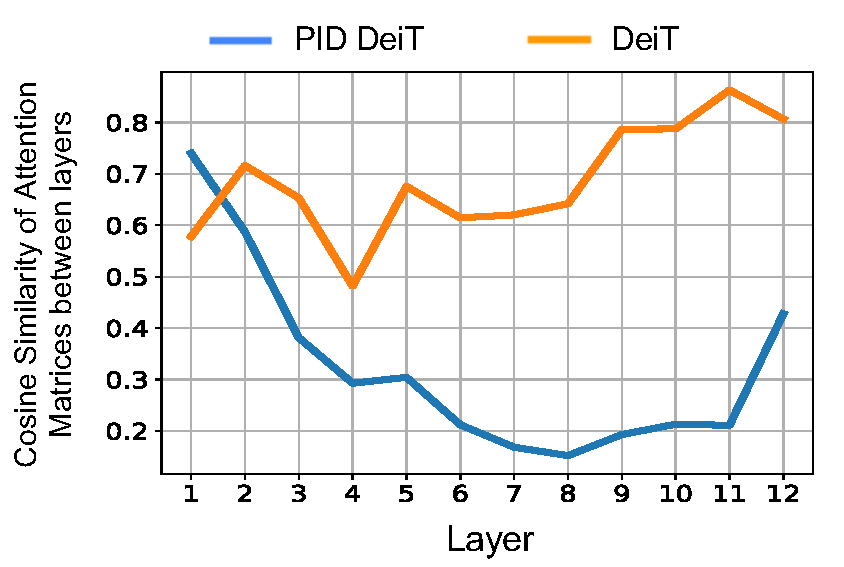
\includegraphics[width=0.38\textwidth]{iclr_2023/pictures/pidrank-collapse.pdf}
\vspace{-3mm}
\caption{\small The cosine \textit{similarity} of token representations in PID DeiT compared to baseline DeiT models across layers for ImageNet classification. The DeiT baseline demonstrates representation rank collapse as tokens become increasingly similar as depth increases. In contrast, PID DeiT models exhibit significantly greater diversity in tokens, indicating a mitigation in rank-collapse.}
\label{fig:pid-cossim} 
% \vspace{-0.in}
\end{figure}